%%%%%%%%%%%%%%%%%%%%%%%%%%%%%%%%%%%%%%%%%
% Journal Article
% LaTeX Template
% Version 2.0 (February 7, 2023)
%
% This template originates from:
% https://www.LaTeXTemplates.com
%
% Author:
% Vel (vel@latextemplates.com)
%
% License:
% CC BY-NC-SA 4.0 (https://creativecommons.org/licenses/by-nc-sa/4.0/)
%
% NOTE: The bibliography needs to be compiled using the biber engine.
%
%%%%%%%%%%%%%%%%%%%%%%%%%%%%%%%%%%%%%%%%%

%----------------------------------------------------------------------------------------
%	PACKAGES AND OTHER DOCUMENT CONFIGURATIONS
%----------------------------------------------------------------------------------------

\documentclass[
	a4paper, % Paper size, use either a4paper or letterpaper
	10pt, % Default font size, can also use 11pt or 12pt, although this is not recommended
	unnumberedsections, % Comment to enable section numbering
	twoside, % Two side traditional mode where headers and footers change between odd and even pages, comment this option to make them fixed
]{LTJournalArticle}

\addbibresource{sample.bib} % BibLaTeX bibliography file

\runninghead{GEVIS: A Differential Gene Expression Analysis Web-Application Tool for Lung Adenocarcinoma} % A shortened article title to appear in the running head, leave this command empty for no running head

\footertext{\textit{Cristian Santaroni, Francesco Fortunato} (March 2024)} % Text to appear in the footer, leave this command empty for no footer text

\setcounter{page}{1} % The page number of the first page, set this to a higher number if the article is to be part of an issue or larger work

%----------------------------------------------------------------------------------------
%	TITLE SECTION
%----------------------------------------------------------------------------------------

\title{GEVIS: \\A Differential Gene Expression Analysis Web-Application Tool for Lung Adenocarcinoma
} % Article title, use manual lines breaks (\\) to beautify the layout

% Authors are listed in a comma-separated list with superscript numbers indicating affiliations
% \thanks{} is used for any text that should be placed in a footnote on the first page, such as the corresponding author's email, journal acceptance dates, a copyright/license notice, keywords, etc
\author{%
	Cristian Santaroni, Francesco Fortunato 
}

% Affiliations are output in the \date{} command
\date{\footnotesize University of Rome ``Sapienza''\\ Department of Ingegneria Informatica, Automatica e Gestionale ``Antonio Ruberti''\\ Visual Analytics Course, Master's Degree in Engineering in Computer Science}

% Full-width abstract
\renewcommand{\maketitlehookd}{%
	\begin{abstract}
            \noindent Our presented dashboard emerges as a tool aimed at addressing the critical needs of bioinformaticians, medical professionals, and researchers in unraveling the complexities of gene expression data. Motivated by the importance of precision medicine, our platform integrates statistical analyses and intuitive visualizations to facilitate in-depth exploration of differential gene expression patterns. Gene expression, serves as a cornerstone in understanding molecular mechanisms underlying various diseases and timely and accurate interpretation of gene expression data is crucial in the context of personalized medicine and diagnostic advancements.
	\end{abstract}
}

%----------------------------------------------------------------------------------------

\begin{document}

\maketitle % Output the title section

%----------------------------------------------------------------------------------------
%	ARTICLE CONTENTS
%----------------------------------------------------------------------------------------

\section{Introduction}

Gene expression analysis stands as a cornerstone in modern molecular biology, providing invaluable insights into the intricate mechanisms governing cellular processes, development, and disease \cite{rosati2024differential}. As the fundamental link between genomic information and functional outcomes, the study of gene expression elucidates the dynamic interplay of genetic elements within an organism.

In recent years, advancements in high-throughput technologies have revolutionized the scale and depth of gene expression profiling, enabling the simultaneous measurement of thousands of genes across diverse biological samples. This surge in data complexity has necessitated the development of sophisticated analytical tools and frameworks to extract meaningful information from large-scale expression datasets. 

Understanding gene expression patterns holds profound implications for numerous fields, ranging from basic research to clinical applications. In the realm of basic science, gene expression analysis serves as a compass guiding researchers through the exploration of cellular responses to stimuli, developmental transitions, and the intricacies of cellular communication. Concurrently, the clinical relevance of gene expression analysis has become increasingly apparent, with applications spanning disease diagnosis, prognosis, and the identification of therapeutic targets \cite{rosati2024differential}.

%------------------------------------------------

\section{Study Background and Dataset Description}


\subsection{Purpose of the Study}
Tobacco use is the largest preventable cause of cancer and cancer mortality, responsible for approximately one-third of all cancer deaths annually. Sufficient evidence has been accumulated to infer a causal relationship between tobacco use and cancers of the lung, larynx, oral cavity, pharynx, esophagus, pancreas, bladder, kidney, cervix, stomach, and acute myeloid leukemia, with additional evidence suggesting a causal relationship for colorectal and liver cancer. There are more than 60 known or suspected carcinogens in cigarette smoke that form DNA adducts and mutations, leading to loss of normal growth control mechanisms. In addition to substantial cancer risks, tobacco use also increases risk for other life-threatening chronic illnesses, including cardiovascular disease, stroke, pulmonary disease, and adverse health effects.


\subsection{Dataset Overview}
In our pursuit to elucidate the elusive molecular alterations induced by tobacco smoking in the development of lung cancer and their impact on survival, we conduct a gene expression analysis utilizing the GSE10072 dataset. The GSE10072 dataset, originates from the Gene Expression Omnibus (GEO), a public repository hosted by the National Center for Biotechnology Information (NCBI) which serves as a centralized hub for high-throughput functional genomics data, offering researchers a diverse array of datasets to facilitate scientific inquiry. 

The GSE10072 dataset specifically focuses on lung tissues, providing a comprehensive collection of gene expression profiles obtained through microarray technology. This dataset comprises samples from both individuals with lung cancer and those without, allowing for a comparative analysis between cancerous and normal lung tissues. 

Structured as a matrix, the GSE10072 dataset features rows corresponding to individual genes, metadata and columns representing distinct samples. For each entry in the matrix, the gene expression level is quantified, capturing the intensity of gene activity within the respective lung tissue sample. Notably, the dataset includes information about the smoker class, the gender, the stage, and the age for each sample.


%------------------------------------------------

\section{Differential Expressed Genes Analysis}

Identifying genes exhibiting significant expression changes between conditions (normal vs tumor) is the main goal of the DEG analysis \cite{rosati2024differential}. It involves preliminary steps like pre-processing the entire dataset to make it more suitable for further operation that are the core part of DEG \cite{rosati2024differential}. By subjecting this dataset to rigorous gene expression analysis techniques, we aim to identify key molecular signatures associated with tobacco or gene-induced alterations in lung tissues that may contribute to the initiation and progression of lung cancer. 

The steps in details are:
\begin{itemize}
    \item \textbf{Pre-processing}: Data are pre-processed through a R Studio script. We apply a logarithmic transformation to the expression values to stabilize variance and meet the assumptions of downstream statistical analyses. This transformation helps to make the data more symmetric and reduces the influence of extreme values.
    \item \textbf{Computing of variation and filtering}: The interquartile range (IQR) is calculated for each gene to measure the variation around the median expression level. Genes with low variation (below a specified threshold) are filtered out to focus on those showing significant expression changes between conditions. This method is inspired by the work of Chockalingam et al. (2016) \cite{chockalingam2016microarray}, where the IQR threshold is visually selected by identifying the histogram bin with the highest number of genes, ensuring that the selected threshold reflects the dataset's characteristic variability of expression values.
\item \textbf{Computing of Log Fold Change and filtering}: The magnitude of change in gene expression between conditions is also considered: Log Fold Change (LogFC) is calculated as the logarithm (base 2) of the ratio of the mean expression levels between case and control samples for each gene. 
    \begin{itemize}
        \item Genes with \textbf{LogFC $>$ 0 }indicate an increase in expression in case samples compared to control samples. Those genes are commonly said to be \textbf{up-regulated} in case group.
        \item Genes with \textbf{LogFC $<$ 0} indicate a decrease in expression in case samples compared to control samples. Those genes are commonly said to be \textbf{down-regulated} in case group.
    \end{itemize}
    The method proposed by McCarthy and al. (2009) \cite{mccarthy2009testing} supports the use of Log Fold Change as a measure for assessing the magnitude of differential expression in microarray experiments, but in concomitance of a statistical testing.
    
\item \textbf{Statistical testing}: Using the t-test, we can identify genes that show significant differences in expression levels between conditions. To explain the statistical significance of the results of the statistical test, it is used the significance level. It is the \textbf{probability to reject the null hypothesis when it is assumed to be true } and using 0.05 or 0.01 as a significance level indicates a 5$\%$ (1$\%$) risk of concluding that a difference exists when there is no actual difference.
    
\item \textbf{Multiple Testing Correction}: Since thousands of genes are tested simultaneously, multiple testing correction methods such as the false discovery rate (FDR), correction are applied to control for false positives. The combination of these methods is supported by the ad hoc approach presented by McCarthy and al. (2009) \cite{mccarthy2009testing}, where they propose methods like the TREAT (t-tests relative to a threshold), which formalizes the assessment of differential expression considering both fold-change and statistical significance. 

\item \textbf{Principal Component Analysis}: In our analysis of Differential Expressed Genes (DEGs), we employed Principal Component Analysis (PCA) to visualize the relationships between samples and identify potential clusters or groups based on their expression profiles. We chose PCA due to its effectiveness in dimension reduction and its ability to capture variation in high-dimensional gene expression data. PCA has been widely applied in bioinformatics studies, including gene expression analysis, due to its simplicity, computational efficiency, and ability to provide insights into complex datasets (Ma et al., 2011) \cite{ma2011principal}. Additionally, PCA allows for exploratory analysis, data visualization, clustering, and regression analysis, making it a versatile tool for understanding gene expression patterns and relationships among samples \cite{ma2011principal}.
    
\end{itemize}


\section{Related Works}
There are many visualization tools that are available in the literature, which allow to perform a gene expression analysis. We have decided to take into account some of them which we consider to be the most suitable to perform this analysis.

The first example tool is the web application called Phantasus \cite{Kleverov2022.12.10.519861}. While this solution differs in presentation from ours, the underlying concept is essentially the same. Like our platform, Phantasus allows users to perform preprocessing operations such as adjusting expression values on a logarithmic scale and eliminating genes with low expression profiles. However, a notable distinction is that Phantasus provides users with the option to skip the preprocessing step entirely, which we believe is crucial for ensuring the reliability of subsequent analyses. Additionally, our approach involves selecting IQR and LogFC values through visualization of graphs, a step that Phantasus does not incorporate. This visualization-driven approach enables users to make informed decisions about these parameters, enhancing the accuracy and relevance of their analyses.

One of the commonly used methods to visualize metadata associated with samples, such as cancer stage, smoker status, age, and gender, is through heatmaps, as seen in tools like Phantasus. While heatmaps offer a convenient way to display the entire dataset, including genes, samples, and metadata, there is a risk of losing focus on relevant genes due to the heatmap occupying most of the screen space. To address this issue, we opted to separate the visualization of metadata from the complete set of genes by employing parallel coordinates. This approach allows users to examine the relationships between patients, their metadata, and selected relevant genes, without overwhelming them with excessive information. Additionally, by integrating features like box plots and scatterplots within the same interface, we eliminate the need for multiple windows or additional charts, ensuring a seamless and comprehensive analysis experience.


Certainly, an advanced tool should be capable of accepting input from various datasets representing different diseases. This functionality is well-implemented in the solution we have mentioned, but also in Network Analyst \cite{10.1093/nar/gkz240}. Network Analyst offers gene expression analysis in a manner similar to ours, providing direct visualization of differentially expressed genes through a volcano plot. This visualization aids in understanding which genes are filtered based on both logFC and p-value criteria. While Network Analyst utilizes a volcano plot for visualizing differentially expressed genes, we made a deliberate choice to employ a scatterplot instead in our tool. This decision was based on several considerations. Firstly, scatterplots offer a more intuitive representation of gene expression data, allowing users to directly contrast the logarithmic mean expression level in the normal group against the logarithmic mean expression level in the case group. This straightforward visualization facilitates the identification of genes that exhibit substantial changes in expression levels with statistical significance. Additionally, scatterplots provide a flexible platform for interactive exploration, enabling users to select genes of interest and dynamically adjust visualization parameters. This versatility enhances user engagement and promotes a deeper understanding of the data. However, Network Analyst also incorporates analyses not present in our tool, such as molecular interaction analysis. Despite its strengths, Network Analyst lacks certain features that could enhance its utility. For instance, it does not provide information about the contribution of genes to principal components, and it lacks a parallel coordinate plot, which could offer valuable insights into the data.

\begin{figure*} % Two column figure (notice the starred environment)
	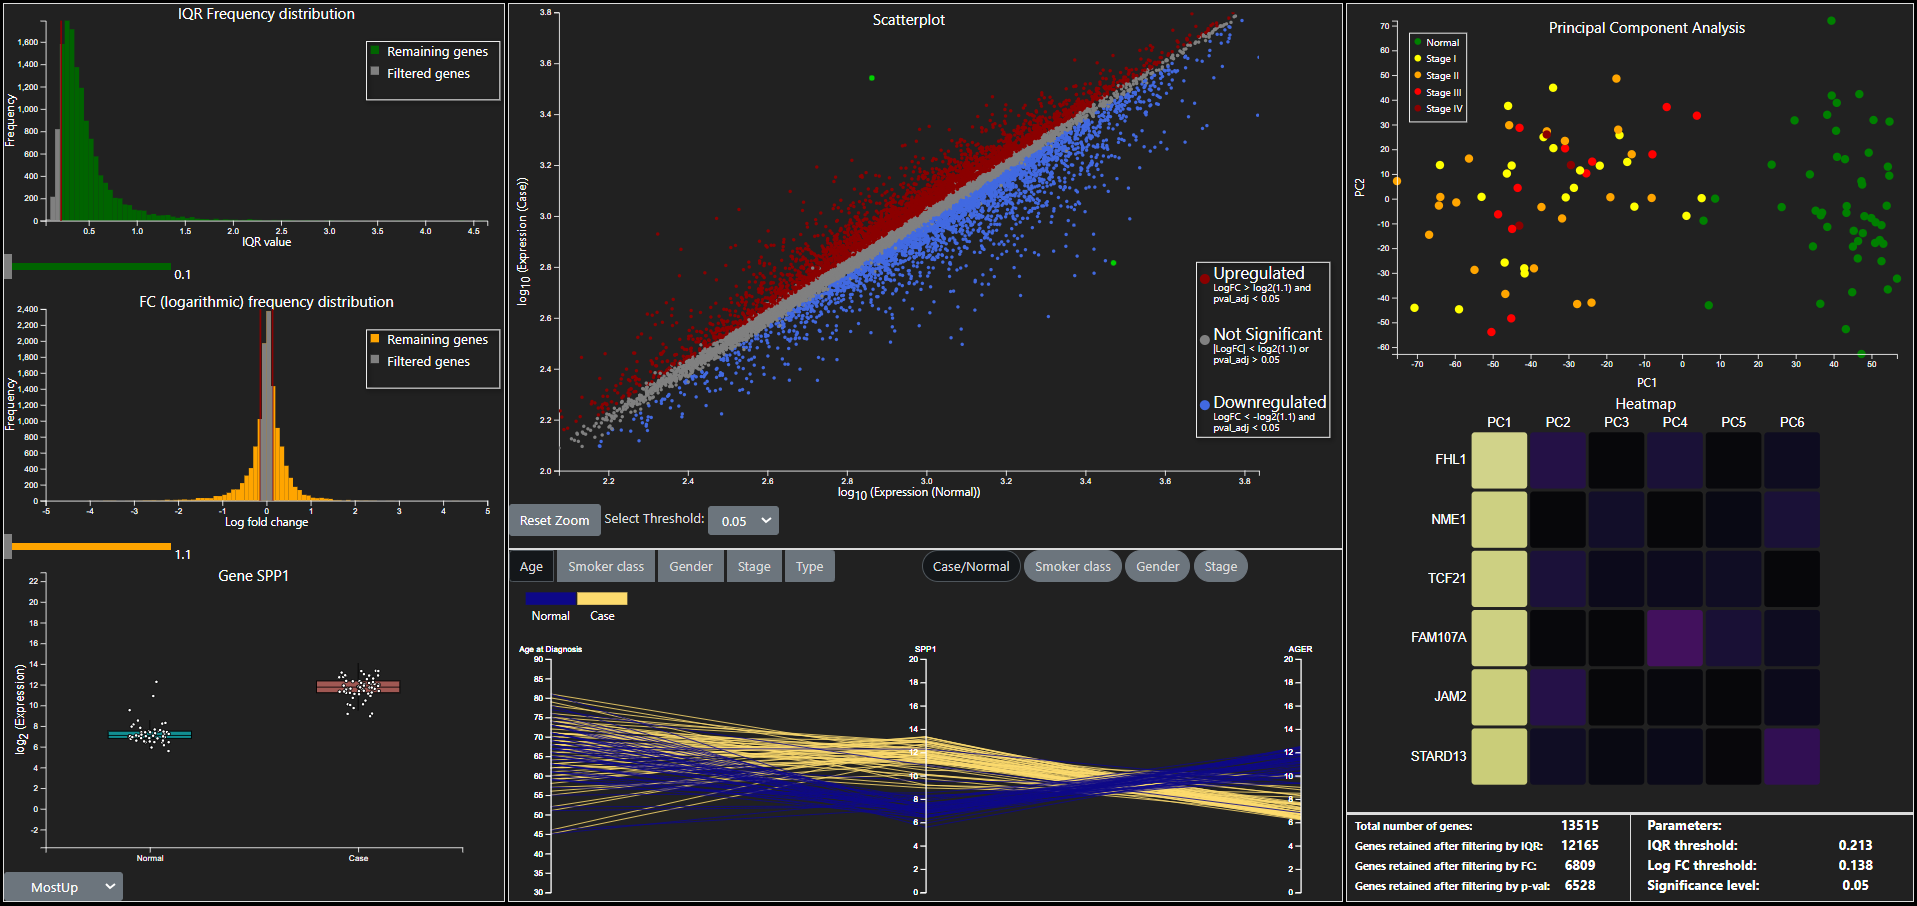
\includegraphics[width=\linewidth]{Figures/GEVIS Dashboard.png}
	\caption{A screenshot of GEVIS dashboard. The dashboard features several visualizations for differential gene expression analysis. The top left panel displays IQR and logarithmic Fold-Change frequency distributions for remaining genes and filtered genes. In the top middle panel, a scatterplot contrasts gene expression ($log_{10}$) between normal and cancer samples. The top right panel presents a multicolored (according to the stage) PCA plot, revealing clusters within the data. Below the PCA plot, a heatmap illustrates  variable contributions of genes to principal components computed through PCA analysis (PC1 to PC6). The bottom left corner represents the boxplot of the selected gene. The bottom middle section features a parallel coordinate graph. The bottom right corner provides essential statistics, including the total number of genes, genes retained after filtering by IQR, fold change (FC), p-value and other parameters such as IQR, LogFC and p-value thresholds.}
	\label{fig:gevis_dashboard}
\end{figure*}


\section{Overview of the Visualization System}

Our proposed system, GEVIS - Gene Expression VIS, is a comprehensive dashboard designed to facilitate differential gene expression analysis. GEVIS provides researchers with an intuitive and interactive platform for exploring gene expression data, identifying differentially expressed genes, and gaining insights into underlying biological mechanisms.

At the core of GEVIS is a series of visualization tools and statistical analyses that enable users to conduct differential expression analysis on the GSE10072 dataset and visualize the results in real-time. The system incorporates various visualization techniques, including histograms, scatterplots, boxplots, parallel coordinates graph and principal component analysis (PCA), to facilitate a comprehensive understanding of complex gene expression patterns, enabling researchers to discern subtle trends and uncover significant insights.

One of the key features of GEVIS is its seamless integration of multiple views, allowing users to interact with their data from different perspectives simultaneously. For example, users can explore gene expression profiles using scatterplots while also examining the distribution of expression values across samples using boxplots. This multidimensional approach enhances the user's ability to detect subtle changes in gene expression and uncover potential biomarkers or therapeutic targets.

In addition to visualization tools, GEVIS also includes interactive features such as sliders for selecting IQR and LogFC thresholds, dropdown menus for adjusting parameters, and filtering results dynamically. This flexibility empowers researchers to tailor their analyses to specific research questions and explore different hypotheses with ease.

The overall layout and functionality of GEVIS are depicted in Figure \ref{fig:gevis_dashboard}, which showcases a screenshot of the GEVIS dashboard.

\subsection{IQR (Interquartile Range)}

The IQR (Interquartile Range) graph in GEVIS provides users with a visual representation of the distribution of gene expression values within the dataset. By adjusting the slider for the interquartile range, users can filter genes based on their variability across samples \cite{chockalingam2016microarray}. This allows researchers to focus on genes with significant variability and potential biological relevance, aiding in the identification of differentially expressed genes.

\subsection{LogFC (Logarithmic Fold Change)}

The LogFC (Logarithmic Fold Change) graph displays the distribution of fold changes in gene expression between case and normal samples. Users can adjust the log threshold slider to filter genes based on their fold change values \cite{mccarthy2009testing}.

\subsection{Scatterplot}

In GEVIS, the scatterplot serves as a powerful visualization tool for exploring gene expression patterns between different sample groups. Each data point on the scatterplot represents a gene, with the logarithmic mean expression level in the normal group plotted against the logarithmic mean expression level in the case group.

The scatterplot enables researchers to quickly identify genes that exhibit significant changes in expression between the two groups. Genes colored in red indicate upregulated expression in the case group compared to the normal group, while those in blue represent downregulated expression. Additionally, genes colored in grey signify either filtered-out genes based on the logFC threshold or those not deemed statistically significant (p-value above a predefined threshold).

An interactive feature of the scatterplot allows users to click on individual genes of interest. Upon selection, an animation highlights the chosen gene, providing immediate visual feedback. Furthermore, clicking on a gene triggers the addition of a corresponding axis in the scatterplot, visually representing the gene's expression levels. Additionally, the selected gene is dynamically added to the dropdown menu in the boxplot section, facilitating further analysis and exploration. Finally, when users move the mouse on a gene, a tooltip will be displayed, showing several attributes of that gene such as its name, LogFC, p-value, mean expression in case and normal samples.

\subsection{Boxplot}

The boxplot graph in GEVIS displays the distribution of gene expression values across case and normal samples for selected genes. A dropdown menu provides easy access to select specific genes of interest, allowing researchers to compare expression levels across sample groups systematically. Users can interactively select genes from the scatterplot, and the corresponding gene will be added dinamically to the dropdown menu. This allows users to visualize the variability in gene expression between sample groups and identify potential outliers or patterns.

Moreover, we enhanced user interaction by enabling highlighting of corresponding lines in the parallel coordinate plot when clicking on jitters in the boxplot to facilitates seamless exploration of gene expression data across multiple visualization views, allowing researchers to identify patterns and correlations effectively.

\subsection{Parallel Coordinates}

In the parallel coordinate graph of GEVIS, each line represents a sample (person), while the axes represent both metadata and genes. Users have the flexibility to add or remove metadata categories such as age, gender, type (case/normal), smoker class (current smoker, former smoker, never smoked), and stage. Additionally, users can customize the encoding of the lines based on metadata categories, allowing for visual comparisons across different attributes.

An essential feature of the parallel coordinate graph is the ability for users to dynamically add or remove genes by selecting them from other visualization components, such as the scatterplot. This enables researchers to focus on specific genes of interest and explore their relationships with metadata attributes.

Furthermore, users can rearrange the order of the axes, providing flexibility in data exploration and facilitating the identification of patterns and correlations. This interactive feature allows researchers to tailor the visualization to their specific research questions and hypotheses.

Additionally, GEVIS supports seamless interaction between different visualization components. Users can click on a path in the parallel coordinate graph to highlight the corresponding sample, which is then highlighted in other visualization components such as boxplots and PCA plots. Similarly, clicking on a jitter in the boxplot or brushing a point in the PCA plot highlights the corresponding sample in the parallel coordinate graph, facilitating cross-referencing and deeper exploration of the data.

\subsection{PCA (Principal Component Analysis)}

GEVIS employs PCA to visualize high-dimensional gene expression data in a lower-dimensional space, facilitating the detection of patterns and clusters among samples. The PCA plot provides an interactive platform where users can explore relationships between samples and identify groups or outliers based on gene expression profiles. We enhanced user interaction by implementing brushing functionality, allowing researchers to highlight selected paths in the parallel coordinate plot and corresponding jitters in the boxplot. Moreover, PCA incorporates color encoding to represent metadata such as cancer stage, with green indicating normal samples, yellow for stage I, orange for stage II, red for stage III, and dark red for stage IV. This intuitive color scheme enables users to quickly identify sample characteristics and discern meaningful insights from the PCA visualization.
Incorporating a draggable legend for the PCA was a deliberate choice. This feature ensures that, even when adjustments are made to thresholds resulting in changes to the graph, the legend remains accessible and can be repositioned by users for optimal visibility and convenience.


\subsection{Heatmap of Gene Contributions to Principal Components}

In GEVIS, the heatmap serves as a visualization tool to illustrate the contribution percentage of genes to each principal component derived from PCA analysis. Despite its name, this heatmap specifically focuses on showcasing the variable contributions of genes rather than traditional heatmap functionalities. Each square within the heatmap corresponds to a gene's contribution to a principal component, with lighter shades indicating higher contribution percentages.

Users can interact with the heatmap by selecting squares, triggering the highlighting of corresponding data points in the scatterplot. The color of the highlighted points in the scatterplot is encoded based on the value of the selected gene with respect to a specific principal component. Additionally, it incorporates a tooltip feature that displays the value of each square upon hovering, facilitating a detailed examination of gene contributions to principal components. This interactive visualization tool provides researchers with valuable insights into the underlying structure of gene expression data and helps identify key genes driving sample clustering and variability.

\section{Technology Stack}

GEVIS utilize a combination of technologies and tools to facilitate various aspects of the gene expression analysis process. Below, we provide a detailed overview of the technologies employed:

\begin{itemize}
    \item \textbf{Node.js}: Node.js served as the foundation for our server-side operations, providing a robust runtime environment for executing JavaScript code. 
    
    \item \textbf{HTML with D3.js}: HTML, coupled with D3.js (Data-Driven Documents), formed the backbone of our client-side visualization system. D3.js is a powerful JavaScript library that enables the creation of dynamic and interactive visualizations directly within the web browser. Through HTML and D3.js, we developed custom visualizations and user interactions for exploring gene expression data in an intuitive manner.
    
    \item \textbf{RStudio}: RStudio played a crucial role in conducting initial preprocessing and transformations of the gene expression data. Leveraging R packages such as GEOquery, we were able to download, process, and analyze datasets from the GEO database. We first extracted metadata. Then, we removed those genes with a overall mean of 0, we applied a logarithmic transformation, and we compute IQR for each gene. Finally, we exported the logarithmic transformed data, the metadata, and the IQR for each gene.
    
    \item \textbf{Docker (OpenCPU/RStudio)}: Docker, specifically utilizing the OpenCPU/RStudio image, provided an encapsulated environment for executing R scripts and conducting statistical analyses. This containerization of our analysis pipeline ensured reproducibility and scalability, facilitating seamless deployment across diverse computing environments. Notably, leveraging OCPU enabled us to create APIs (Application Programming Interfaces) for our R scripts, enabling RESTful interaction. This functionality allowed us to execute various analyses, including t-tests for comparing expression levels between groups, applying false discovery rate (FDR) correction to resulting p-values, conducting PCA, and calculating variable contributions for individual genes.
\end{itemize}

The code and instructions for running the analysis pipeline can be found at: \url{https://github.com/francesco-fortunato/GEVIS}.

\section{Results}

The analysis of gene expression data through GEVIS revealed intriguing insights into potential biomarkers for lung adenocarcinoma (LUAD). Among the genes examined, secreted phosphoprotein 1 (SPP1) emerged as the most upregulated gene, while advanced glycosylation end-product specific receptor (AGER) was identified as the most downregulated gene.

This finding holds significant implications for LUAD prognosis and treatment. Research conducted by Zhang et al. (2018) \autocite{Zhang:spp1} supports our discovery, highlighting the prognostic significance of SPP1 and AGER in LUAD. The study identified SPP1 as highly expressed and AGER as lowly expressed in tumor tissues, suggesting their association with LUAD progression and patient survival.

SPP1, known for promoting cancer cell survival and regulating tumor-associated angiogenesis and inflammation, has been implicated in the development and metastasis of lung cancer.

On the other hand, AGER plays a crucial role in diabetic angiopathy and thymic hyperplasia, functioning in toll-like receptor 4 and AGE-RAGE signaling pathways. Its suppression in tumor tissues suggests a potential role in LUAD progression, with high expression levels indicating lung inflammation and exacerbation of other lung diseases. 

Additionally, further examination of scatterplot visualization revealed two other genes, ficolin 3 (FCN3) and transmembrane protein 100 (TMEM100), as potential influencers in lung cancer disease progression. These genes were also identified as follow-ups and candidate common differentially expressed genes in patients with lung adenocarcinoma, along with SPP1 and AGER, by Zhang et al. (2018) \autocite{Zhang:spp1}.

Through our PCA analysis, we identified several genes exhibiting a high contribution percentage in the first component. Upon applying various thresholds and subsequently filtering out differing quantities of genes, two consistently emerged with the highest percentages: FHL1 and TCF21.

Notably, a recent study (Chang et al., 2012) \autocite{Chang:fhl1} showed that FHL1 protein was downregulated in over 90$\%$ of 80 lung cancer patients. Furthermore, experimental manipulation of FHL1 expression levels resulted in a significant suppression of cell proliferation and inhibition of the cell cycle transition between the G1 and G2 phase. Dysregulation in these key stages may lead to aberrant DNA synthesis, genomic instability, and the unchecked proliferation of cells, thereby contributing significantly to the onset and progression of cancer. This implies that reduced expression of FHL1 may play an important role in the development and progression of lung cancer and that FHL1 may be a useful target for lung cancer gene therapy.

Research by Xiao et al. (2017) \autocite{Xiao:TCF21} demonstrated that decreased mRNA expression of TCF21 is an unfavorable prognostic factor for lung adenocarcinoma patients. Their study highlighted the prognostic significance of TCF21 in LUAD, showing that decreased mRNA expression of TCF21 is associated with unfavorable overall survival outcomes for patients with lung adenocarcinoma. This finding further underscores the importance of TCF21 in LUAD prognosis and suggests its potential as a biomarker for identifying high-risk patients.

\section{Conclusions}

In summary, our web tool has provided a platform for gene expression analysis, enabling users to explore, visualize, and derive meaningful insights from their data. However, to further enhance user flexibility and functionality, we envision several potential improvements.

Firstly, future iterations of the tool could incorporate features allowing users to choose between pre-existing datasets for analysis or seamlessly submit and analyze their own datasets. This would broaden the tool's applicability and accommodate diverse research needs.

A critical enhancement could involve automating pre-processing steps to streamline the analysis process. This may include adjusting expression levels based on a logarithmic scale and filtering out genes with low mean expression.

Additionally, the inclusion of hierarchical clustering visualization could be beneficial for identifying groups or clusters of genes with similar expression profiles across different conditions. This feature would provide researchers with valuable insights into the underlying biological processes driving gene expression patterns.

Expanding the tool's capabilities to include gene set annotation and enrichment analysis would significantly enhance its utility. Integrating also survival analysis capabilities would allow users to assess the impact of gene expression on patient survival outcomes. This additions would enable users to gain deeper insights into the biological context of their findings and understand the functional implications associated with differentially expressed genes.

In conclusion, by implementing these enhancements, our web tool could become an even more powerful resource for researchers conducting gene expression analysis, facilitating a deeper understanding of molecular mechanisms underlying various biological phenomena.



%----------------------------------------------------------------------------------------
%	 REFERENCES
%----------------------------------------------------------------------------------------

\printbibliography % Output the bibliography

%----------------------------------------------------------------------------------------

\end{document}
